\newpage
\section{Theory and Implementation} \label{sec:theory}

\begin{figure}[!hrt]
  \centering
  \label{cavity_eom_pdh}
  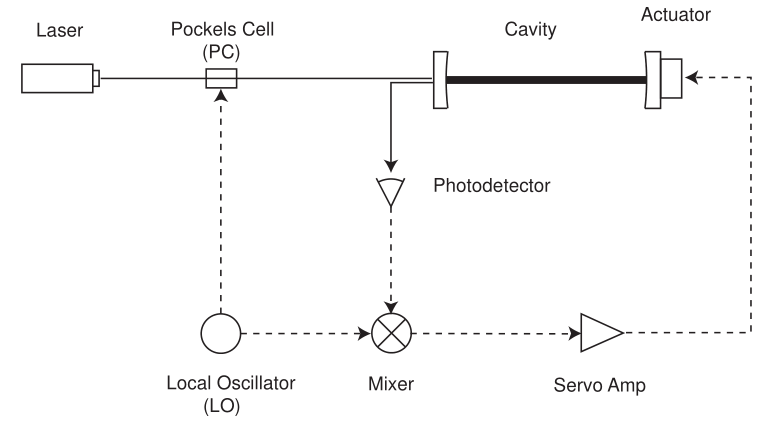
\includegraphics[scale=0.5]{cavity_eom_pdh.png}
  \caption{High level layout of PDH servo loop using an actuated cavity as
  the frequency selective element. Borrowed from \cite{black1998}}
\end{figure}

\begin{figure}[!hrt]
  \centering
  \label{vapour_eom_pdh}
  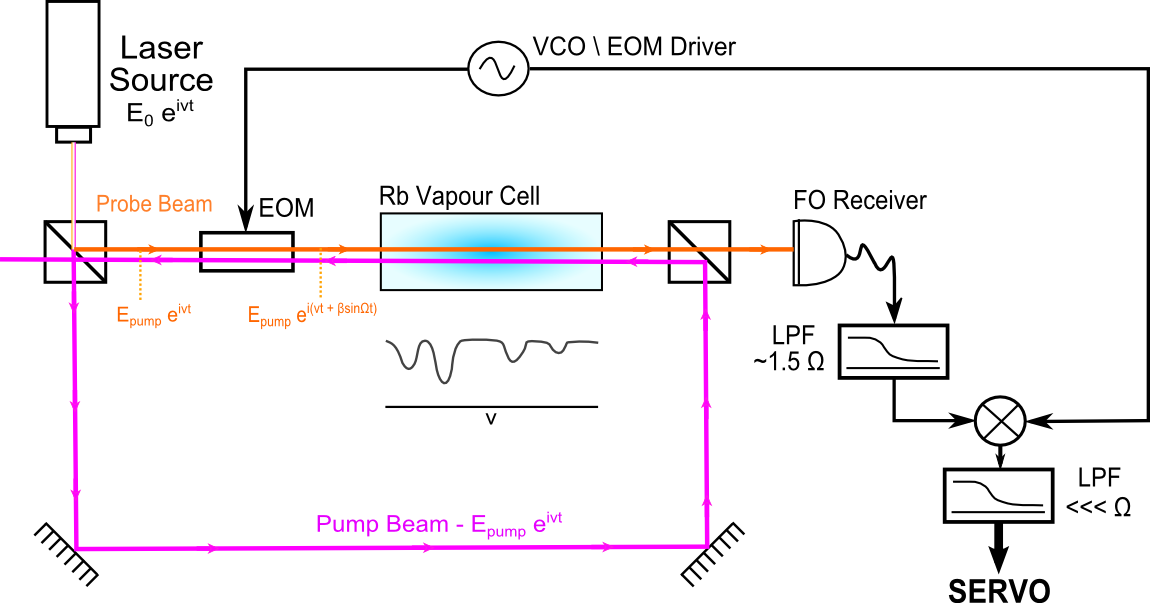
\includegraphics[scale=0.9]{EOM_PDH_UNIT.png}
  \caption{High level layout of PDH servo loop using a Rubidium vapour cell as
  the frequency selective element.}
\end{figure}

\subsection{Brief Overview of Saturated Absorption Spectra}

Maxwell distribution of speed in z-axis only:
\begin{gather}
  \rho(v_z) = \sqrt{\frac{m}{2\pi k_B T}} e^{\frac{-m v_z^2}{2k_B T}}
\end{gather}

Lorentzian absorption feature, with compensation for doppler shifting:
\begin{gather}
  F(\nu, v_z) = \frac{\Gamma / 2 \pi}{(\nu - \nu_0 + \nu_0 v / c)^2 +
  \Gamma^2 / 4}
\end{gather}

"Optical Depth":
\begin{gather}
  \tau(\nu) = \int_{-\infty}^\infty F(\nu, v_z) \rho(v_z) dv_z
\end{gather}

Transmission ratio:
\begin{gather}
  I(\nu, z) = I_0 e^{-\tau(\nu)\cdot z}
\end{gather}

Terms correcting for accessible population due to pump laser:
\begin{gather}
  S(I_p, \nu, v) = \tau_0 \frac{\nu_0}{c} (P_1 - P_2) =
    \tau_0 \frac{\nu_0}{c} (1 - 2 P_2)
\end{gather}
\begin{gather}
  P_2(I_p, \nu, v) = \frac{ (I_p/I_{sat})/2}{1 + (I_p/I_{sat}) +
    4(\nu - \nu_0 - \nu_0 v/c)^2/\Gamma^2}
\end{gather}
corrected optical depth:
\begin{gather}\label{eq:corr_opt_depth}
  \tau'(\nu) = \int_{-\infty}^\infty S(I_p, \nu) F(\nu, v_z) \rho(v_z) dv_z
\end{gather}

It is obvious that the higher bandwidth of the EOM phase modulation de-facto
allows for optimization for a wider variety of feature sizes. But, more
specifically a closer examination of the saturated absorption spectrum of
Rubidium indicates that this bandwidth is much more appropriate than that of an
AOM. The exact modulation frequency can be tuned ad-hoc to match a particular
optical scheme.

\begin{figure}[!hrt]
  \centering
  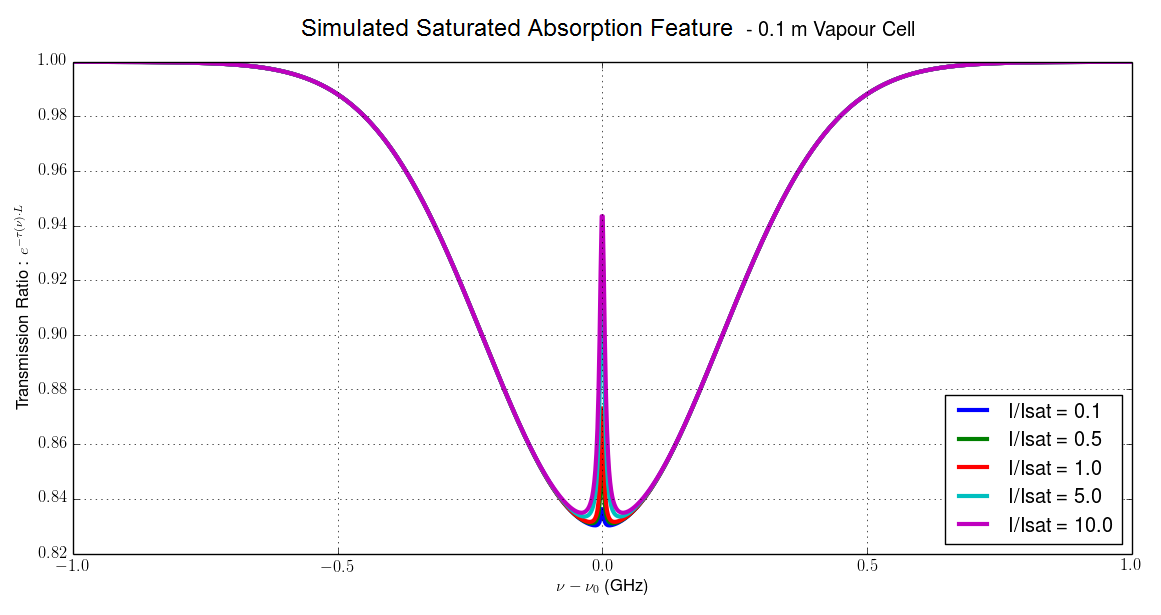
\includegraphics[scale=0.5]{rb_D2_single_absorption.png}
  \caption{Transmission ratio of probe beam through a 0.1m long cell of Rubidium
  gas, near the D2 feature. Optical depth is calculated as shown in
  \textbf{(\ref{eq:corr_opt_depth})},
  and all hyperfine splitting is ignored, (assumed 2-level system) for
  simplicity. The spectrum is plotted for a variety of pump beam intensities
  showing the saturating effect on the velocity classes near $v_z = 0$ at
  resonance.}
  \label{fig:rb87d2abs}
\end{figure}

\begin{figure}[!hrt]
  \centering
  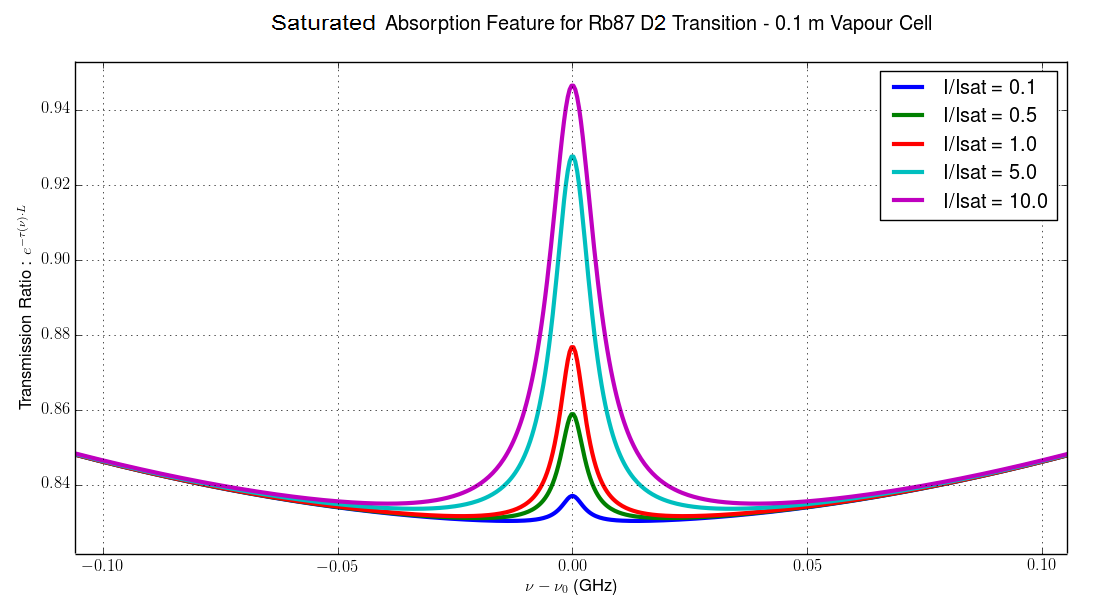
\includegraphics[scale=0.5]{rb_D2_single_absorption_resonance.png}
  \caption{Closer view of \textbf{Figure~\ref{fig:rb87d2abs}}, near the
  resonance.}
  \label{fig:rb87d2abs_closer}
\end{figure}

\subsection{Optical Phase Modulation}

\subsection{Error Signal Generation}

Obtaining an accurate value for the optimal error signal slope will be a central
development task, if it is not possible to optmize heuristically in a way that
is comfortable for the laboratory staff. This will involve some detailed
quantum mechanical analysis, but there are precedents for reference
\cite{maguire2006}

